\documentclass[12pt, titlepage]{article}

\usepackage{fullpage}
\usepackage[round]{natbib}
\usepackage{multirow}
\usepackage{booktabs}
\usepackage{tabularx}
\usepackage{graphicx}
\usepackage{float}
\usepackage{hyperref}
\usepackage{longtable}
\hypersetup{
    colorlinks,
    citecolor=blue,
    filecolor=black,
    linkcolor=red,
    urlcolor=blue
}

%% Comments

\usepackage{color}

\newif\ifcomments\commentstrue %displays comments
%\newif\ifcomments\commentsfalse %so that comments do not display

\ifcomments
\newcommand{\authornote}[3]{\textcolor{#1}{[#3 ---#2]}}
\newcommand{\todo}[1]{\textcolor{red}{[TODO: #1]}}
\else
\newcommand{\authornote}[3]{}
\newcommand{\todo}[1]{}
\fi

\newcommand{\wss}[1]{\authornote{blue}{SS}{#1}} 
\newcommand{\plt}[1]{\authornote{magenta}{TPLT}{#1}} %For explanation of the template
\newcommand{\an}[1]{\authornote{cyan}{Author}{#1}}

%% Common Parts

\newcommand{\progname}{Software Engineering} % PUT YOUR PROGRAM NAME HERE
\newcommand{\authname}{Team \#11, OKKM Insights
\\ Mathew Petronilho
\\ Oleg Glotov
\\ Kyle McMaster
\\ Kartik Chaudhari} % AUTHOR NAMES                  

\usepackage{hyperref}
    \hypersetup{colorlinks=true, linkcolor=blue, citecolor=blue, filecolor=blue,
                urlcolor=blue, unicode=false}
    \urlstyle{same}
                                


\newcounter{acnum}
\newcommand{\actheacnum}{AC\theacnum}
\newcommand{\acref}[1]{AC\ref{#1}}

\newcounter{ucnum}
\newcommand{\uctheucnum}{UC\theucnum}
\newcommand{\uref}[1]{UC\ref{#1}}

\newcounter{mnum}
\newcommand{\mthemnum}{M\themnum}
\newcommand{\mref}[1]{M\ref{#1}}

\begin{document}

\title{Module Guide for \progname{}} 
\author{\authname}
\date{\today}

\maketitle

\pagenumbering{roman}

\section{Revision History}

\begin{tabularx}{\textwidth}{p{3cm}p{2cm}X}
\toprule {\bf Date} & {\bf Version} & {\bf Notes}\\
\midrule
Date 1 & 1.0 & Notes\\
Date 2 & 1.1 & Notes\\
\bottomrule
\end{tabularx}

\newpage

\section{Reference Material}

This section records information for easy reference.

\subsection{Abbreviations and Acronyms}

See SRS Documentation at \wss{https://github.com/OKKM-insights/OKKM.insights/tree/main/docs/SRS}

\newpage

\tableofcontents

\listoftables

\listoffigures

\newpage

\pagenumbering{arabic}

\section{Introduction}

Decomposing a system into modules is a commonly accepted approach to developing
software.  A module is a work assignment for a programmer or programming
team~\citep{ParnasEtAl1984}.  We advocate a decomposition
based on the principle of information hiding~\citep{Parnas1972a}.  This
principle supports design for change, because the ``secrets'' that each module
hides represent likely future changes.  Design for change is valuable in SC,
where modifications are frequent, especially during initial development as the
solution space is explored.  

Our design follows the rules layed out by \citet{ParnasEtAl1984}, as follows:
\begin{itemize}
\item System details that are likely to change independently should be the
  secrets of separate modules.
\item Each data structure is implemented in only one module.
\item Any other program that requires information stored in a module's data
  structures must obtain it by calling access programs belonging to that module.
\end{itemize}

After completing the first stage of the design, the Software Requirements
Specification (SRS), the Module Guide (MG) is developed~\citep{ParnasEtAl1984}. The MG
specifies the modular structure of the system and is intended to allow both
designers and maintainers to easily identify the parts of the software.  The
potential readers of this document are as follows:

\begin{itemize}
\item New project members: This document can be a guide for a new project member
  to easily understand the overall structure and quickly find the
  relevant modules they are searching for.
\item Maintainers: The hierarchical structure of the module guide improves the
  maintainers' understanding when they need to make changes to the system. It is
  important for a maintainer to update the relevant sections of the document
  after changes have been made.
\item Designers: Once the module guide has been written, it can be used to
  check for consistency, feasibility, and flexibility. Designers can verify the
  system in various ways, such as consistency among modules, feasibility of the
  decomposition, and flexibility of the design.
\end{itemize}

The rest of the document is organized as follows. Section
\ref{SecChange} lists the anticipated and unlikely changes of the software
requirements. Section \ref{SecMH} summarizes the module decomposition that
was constructed according to the likely changes. Section \ref{SecConnection}
specifies the connections between the software requirements and the
modules. Section \ref{SecMD} gives a detailed description of the
modules. Section \ref{SecTM} includes two traceability matrices. One checks
the completeness of the design against the requirements provided in the SRS. The
other shows the relation between anticipated changes and the modules. Section
\ref{SecUse} describes the use relation between modules.

\section{Anticipated and Unlikely Changes} \label{SecChange}

This section lists possible changes to the system. According to the likeliness
of the change, the possible changes are classified into two
categories. Anticipated changes are listed in Section \ref{SecAchange}, and
unlikely changes are listed in Section \ref{SecUchange}.

\subsection{Anticipated Changes} \label{SecAchange}

Anticipated changes are the source of the information that is to be hidden
inside the modules. Ideally, changing one of the anticipated changes will only
require changing the one module that hides the associated decision. The approach
adapted here is called design for
change.

\begin{description}
\item[\refstepcounter{acnum} \actheacnum \label{acHardware}:] The specific
  hardware on which the software is running.
\item[\refstepcounter{acnum} \actheacnum \label{acInput}:] The format of the
  initial input data.
\item ...
\end{description}

\wss{Anticipated changes relate to changes that would be made in requirements,
design or implementation choices.  They are not related to changes that are made
at run-time, like the values of parameters.}

\subsection{Unlikely Changes} \label{SecUchange}

The module design should be as general as possible. However, a general system is
more complex. Sometimes this complexity is not necessary. Fixing some design
decisions at the system architecture stage can simplify the software design. If
these decision should later need to be changed, then many parts of the design
will potentially need to be modified. Hence, it is not intended that these
decisions will be changed.

\begin{description}
\item[\refstepcounter{ucnum} \uctheucnum \label{ucIO}:] Input/Output devices
  (Input: File and/or Keyboard, Output: File, Memory, and/or Screen).
\item ...
\end{description}

\section{Module Hierarchy} \label{SecMH}

This section provides an overview of the module design. Modules are summarized
in a hierarchy decomposed by secrets in Table \ref{TblMH}. The modules listed
below, which are leaves in the hierarchy tree, are the modules that will
actually be implemented.

\begin{description}



\item [\refstepcounter{mnum} \mthemnum \label{mHH}:] Hardware-Hiding Module
\item [\refstepcounter{mnum} \mthemnum \label{aci}:]
Account Creation Interface
\item [\refstepcounter{mnum} \mthemnum \label{accdc}:]
Account Database Connector
\item [\refstepcounter{mnum} \mthemnum \label{accd}:]
Account Database
\item [\refstepcounter{mnum} \mthemnum \label{aui}:]
Account Update Interface
\item [\refstepcounter{mnum} \mthemnum \label{li}:]
Login Interface
\item [\refstepcounter{mnum} \mthemnum \label{at}:]
Access Token
\item [\refstepcounter{mnum} \mthemnum \label{labeler}:]
Labeler
\item [\refstepcounter{mnum} \mthemnum \label{client}:]
Client
\item [\refstepcounter{mnum} \mthemnum \label{user}:]
User
\item [\refstepcounter{mnum} \mthemnum \label{acc}:]
Account Creation Controller
\item [\refstepcounter{mnum} \mthemnum \label{auc}:]
Account Update Controller
\item [\refstepcounter{mnum} \mthemnum \label{ac}:]
Authentication Controller
\item [\refstepcounter{mnum} \mthemnum \label{siri}:]
Satellite Image Request Interface
\item [\refstepcounter{mnum} \mthemnum \label{sirc}:]
Satellite Image Request Controller
\item [\refstepcounter{mnum} \mthemnum \label{sirf}:]
Satellite Image Request
\item [\refstepcounter{mnum} \mthemnum \label{pci}:]
Project Creation Interface
\item [\refstepcounter{mnum} \mthemnum \label{pcc}:]
Project Creation Controller
\item [\refstepcounter{mnum} \mthemnum \label{project}:]
Project
\item [\refstepcounter{mnum} \mthemnum \label{srfi}:]
Service Request Failure Interface
\item [\refstepcounter{mnum} \mthemnum \label{iui}:]
Image Upload Interface
\item [\refstepcounter{mnum} \mthemnum \label{ri}:]
Report Interface
\item [\refstepcounter{mnum} \mthemnum \label{rc}:]
Report Controller
\item [\refstepcounter{mnum} \mthemnum \label{report}:]
Report
\item [\refstepcounter{mnum} \mthemnum \label{psi}:]
Project Selection Interface
\item [\refstepcounter{mnum} \mthemnum \label{psc}:]
Project Selection Controller
\item [\refstepcounter{mnum} \mthemnum \label{lbli}:]
Labeling Interface
\item [\refstepcounter{mnum} \mthemnum \label{lblc}:]
Labeling Controller
\item [\refstepcounter{mnum} \mthemnum \label{image}:]
Image
\item [\refstepcounter{mnum} \mthemnum \label{label server}:] Label Server
\item [\refstepcounter{mnum} \mthemnum \label{label database connector}:] Label Database Connector
\item [\refstepcounter{mnum} \mthemnum \label{label database}:] Label Database
\item [\refstepcounter{mnum} \mthemnum \label{ImageObject database connector}:] ImageObject Database Connector
\item [\refstepcounter{mnum} \mthemnum \label{ImageObject database}:] ImageObject Database
\item [\refstepcounter{mnum} \mthemnum \label{Labeller database connector}:] Labeller Database Connector
\item [\refstepcounter{mnum} \mthemnum \label{Labeller database}:] Labeller Database
\item [\refstepcounter{mnum} \mthemnum \label{Object Extraction Manager}:]Object Extraction Manager
\item [\refstepcounter{mnum} \mthemnum \label{Image Service Manager}:]Image Service Manager
\item [\refstepcounter{mnum} \mthemnum \label{Label Confidence Service}:]Label Confidence Service
\item [\refstepcounter{mnum} \mthemnum \label{Object Extraction Service}:]Object Extraction Service
\item [\refstepcounter{mnum} \mthemnum \label{Image Prior Analyzer}:]Image Prior Analyzer
\item [\refstepcounter{mnum} \mthemnum \label{Labeller Expertise Calculator}:]Labeller Expertise Calculator
\item [\refstepcounter{mnum} \mthemnum \label{Image Mask Service}:]Image Mask Service
\item [\refstepcounter{mnum} \mthemnum \label{Image Selection Service}:]Image Selection Service

\end{description}


\begin{table}[h!]
\centering
\begin{tabular}{p{0.3\textwidth} p{0.6\textwidth}}
\toprule
\textbf{Level 1} & \textbf{Level 2}\\
\midrule

{Hardware-Hiding Module} & ~ \\
\midrule




\multirow{7}{0.3\textwidth}{Behaviour-Hiding Module} & Account Creation Interface\\
& Account Database\\
& Account Database Connector\\
& Account Update Interface\\
& Login Interface\\
& Access Token\\
& Labeler\\
& Client\\ 
& User\\
& Satellite Image Request Interface\\
& Satellite Image Request\\
& Project Creation Interface\\
& Project\\
& Service Request Failure Interface\\
& Image Upload Interface\\
& Report Interface\\
& Report\\
& Project Selection Interface\\
& Labeling Interface\\
& Image\\
& Label Server\\
& Label Database Connector\\
& Label Database\\
& ImageObject Database Connector\\
& ImageObject Database\\
& Labeller Database Connector\\
& Labeller Database\\
& Object Extraction Manager\\
& Image Service Manager\\
\midrule

\multirow{3}{0.3\textwidth}{Software Decision Module} & {Account Creation Controller}\\
& Account Update Controller\\
& Authentication Controller\\
& Satellite Image Request Controller\\
& Project Creation Controller\\
& Report Controller\\
& Project Selection Controller\\
& Labeling Controller\\
& Label Confidence Service\\
& Object Extraction Service\\
& Image Prior Analyzer\\
& Labeller Expertise Calculator\\
& Image Mask Service\\
& Image Selection Service\\


\bottomrule

\end{tabular}
\caption{Module Hierarchy}
\label{TblMH}
\end{table}

\section{Connection Between Requirements and Design} \label{SecConnection}

The design of the system is intended to satisfy the requirements developed in
the SRS. In this stage, the system is decomposed into modules. The connection
between requirements and modules is listed in Table~\ref{TblRT}.

There are several key high level design decisions that were made to ensure the requirements outlined in the SRS are met. First, the system has been decomposed into several microservices. These services all connect to 
the same databases, but have the flexibility to operate on their own cadence. Each service can be mirrored by a duplicate service to improve capacity. These decisions are critical to ensuring the speed, uptime, capacity, and latency requirements.
Each of the key algorithms in the system have been encapsulated in their own module. These include the object extraction service, image serving, ML model creation, and report generation, among others. This gives the development team the flexibility to experiment with alternative algorithms, allowing continuous improvement towards performance and accuracy requirements.
The authentication service is designed to meet the authentication requirements by ensuring only approved users can access privileged information.
Every functional requirement is covered by the functionality of a subsystem.

% \wss{The intention of this section is to document decisions that are made
%   ``between'' the requirements and the design.  To satisfy some requirements,
%   design decisions need to be made.  Rather than make these decisions implicit,
%   they are explicitly recorded here.  For instance, if a program has security
%   requirements, a specific design decision may be made to satisfy those
%   requirements with a password.}

\section{Module Decomposition} \label{SecMD}

Modules are decomposed according to the principle of ``information hiding''
proposed by \citet{ParnasEtAl1984}. The \emph{Secrets} field in a module
decomposition is a brief statement of the design decision hidden by the
module. The \emph{Services} field specifies \emph{what} the module will do
without documenting \emph{how} to do it. For each module, a suggestion for the
implementing software is given under the \emph{Implemented By} title. If the
entry is \emph{OS}, this means that the module is provided by the operating
system or by standard programming language libraries.  \emph{\progname{}} means the
module will be implemented by the \progname{} software.

Only the leaf modules in the hierarchy have to be implemented. If a dash
(\emph{--}) is shown, this means that the module is not a leaf and will not have
to be implemented.

\subsection{Hardware Hiding Modules (\mref{mHH})}

\begin{description}
\item[Secrets:]The data structure and algorithm used to implement the virtual
  hardware.
\item[Services:]Serves as a virtual hardware used by the rest of the
  system. This module provides the interface between the hardware and the
  software. So, the system can use it to display outputs or to accept inputs.
\item[Implemented By:] OS
\end{description}

\subsection{Behaviour-Hiding Module}

\begin{description}
\item[Secrets:]The contents of the required behaviours.
\item[Services:]Includes programs that provide externally visible behaviour of
  the system as specified in the software requirements specification (SRS)
  documents. This module serves as a communication layer between the
  hardware-hiding module and the software decision module. The programs in this
  module will need to change if there are changes in the SRS.
\item[Implemented By:] --
\end{description}


\subsubsection{Account Creation Interface (\mref{aci})}

\begin{description}
\item[Secrets:]The design format of the account creation user interface.
\item[Services:] Displays a form to collect user information and submits that information to be processed.
\item[Implemented By:] OrbitWatch
\item[Type of Module:] Abstract Object
\end{description}

\subsubsection{Account Database (\mref{accd})}

\begin{description}
\item[Secrets:] The data structure, storage, and access mechanisms for account related data.
\item[Services:] Can store, insert, update and retrieve user account data.
\item[Implemented By:] OrbitWatch
\item[Type of Module:] Abstract Data Type
\end{description}

\subsubsection{Account Database Connector (\mref{accdc})}

\begin{description}
\item[Secrets:] The database access key and database access algorithms.
\item[Services:] Can request storage, insertion, updates and retrieval of user account data from the database.
\item[Implemented By:] OrbitWatch
\item[Type of Module:] Abstract Data Type
\end{description}

\subsubsection{Account Update Interface (\mref{aui})}

\begin{description}
\item[Secrets:]The design format of the update account information user interface.
\item[Services:] Displays a form with the users current information that can be modified and submits any updated information to be processed.
\item[Implemented By:] OrbitWatch
\item[Type of Module:] Abstract Object
\end{description}

\subsubsection{Login Interface (\mref{li})}

\begin{description}
\item[Secrets:]The design format of the login user interface.
\item[Services:] Displays a form to collect login credentials and submits that information to be processed.
\item[Implemented By:] OrbitWatch
\item[Type of Module:] Abstract Object
\end{description}

\subsubsection{Access Token (\mref{at})}

\begin{description}
\item[Secrets:] Token structure, encryption, expiration, and renewal mechanisms.
\item[Services:] Can determine if a user's token has expired and allows the token to be renewed.
\item[Implemented By:] OrbitWatch
\item[Type of Module:] Abstract Data Type
\end{description}

\subsubsection{Labeler (\mref{labeler})}

\begin{description}
\item[Secrets:]The format and structure of Labeler data.
\item[Services:] Takes in the necessary data to create a Labeler.
\item[Implemented By:] OrbitWatch
\item[Type of Module:] Record
\end{description}

\subsubsection{Client (\mref{client})}

\begin{description}
\item[Secrets:]The format and structure of Client data.
\item[Services:] Takes in the necessary data to create a Client.
\item[Implemented By:] OrbitWatch
\item[Type of Module:] Record
\end{description}

\subsubsection{User (\mref{user})}

\begin{description}
\item[Secrets:]The format and structure of User data.
\item[Services:] Takes in the necessary data to create a User.
\item[Implemented By:] OrbitWatch
\item[Type of Module:] Record
\end{description}

\subsubsection{Satellite Image Request Interface (\mref{siri})}

\begin{description}
\item[Secrets:]The design format of the interface for requesting satellite images.
\item[Services:] Displays a form to collect specifics on the satellite images, calculates estimated cost based on current form entries and submits the form information to be processed.
\item[Implemented By:] OrbitWatch
\item[Type of Module:] Abstract Object
\end{description}

\subsubsection{Satellite Image Request (\mref{sirf})}

\begin{description}
\item[Secrets:]The format and structure of the data needed for a satellite image request.
\item[Services:] Takes in the necessary data to create a satellite image request.
\item[Implemented By:] OrbitWatch
\item[Type of Module:] Record
\end{description}

\subsubsection{Project Creation Interface (\mref{pci})}

\begin{description}
\item[Secrets:]The design format of the project creation interface.
\item[Services:] Displays a form to collect project details, calculates an estimated cost using these details and submits that information to be processed.
\item[Implemented By:] OrbitWatch
\item[Type of Module:] Abstract Object
\end{description}

\subsubsection{Project (\mref{project})}

\begin{description}
\item[Secrets:]The format and structure of the data needed for a Project.
\item[Services:] Takes in the necessary data to create a Project.
\item[Implemented By:] OrbitWatch
\item[Type of Module:] Record
\end{description}

\subsubsection{Service Request Failure Interface (\mref{srfi})}

\begin{description}
\item[Secrets:]The design format of the request failure interface.
\item[Services:] Displays a warning to users that something went wrong.
\item[Implemented By:] OrbitWatch
\item[Type of Module:] Abstract Object
\end{description}

\subsubsection{Image Upload Interface (\mref{iui})}

\begin{description}
\item[Secrets:]The design format of the image upload interface.
\item[Services:] Allows users to upload images from their device, and validates they are images of the correct format.
\item[Implemented By:] OrbitWatch
\item[Type of Module:] Abstract Object
\end{description}

\subsubsection{Report Interface (\mref{ri})}

\begin{description}
\item[Secrets:]The design format of the summary report interface.
\item[Services:] Displays statistics and results of a specific project.
\item[Implemented By:] OrbitWatch
\item[Type of Module:] Abstract Object
\end{description}

\subsubsection{Report (\mref{report})}

\begin{description}
\item[Secrets:]The format and structure of Report data.
\item[Services:] Takes in the necessary data to create a Report.
\item[Implemented By:] OrbitWatch
\item[Type of Module:] Record
\end{description}

\subsubsection{Project Selection Interface (\mref{psi})}
\begin{description}
\item[Secrets:]The design format of the project selection interface.
\item[Services:] Display all available projects that a user can label images from.
\item[Implemented By:] OrbitWatch
\item[Type of Module:] Abstract Object
\end{description}

\subsubsection{Labeling Interface (\mref{lbli})}
\begin{description}
\item[Secrets:] The design format of the labeling interface.
\item[Services:] Displays an image to be labeled, displays label choices which can be selected, and allows images to be skipped.
\item[Implemented By:] OrbitWatch
\item[Type of Module:] Abstract Object
\end{description}

\subsubsection{Image (\mref{image})}

\begin{description}
\item[Secrets:]The format and structure of Image data.
\item[Services:] Takes in the necessary data to create a Image.
\item[Implemented By:] OrbitWatch
\item[Type of Module:] Record
\end{description}

\subsubsection{Label Server (\ref{label server})} 
\begin{description}
  \item[Secrets:] The steps to accept and store a label.
  \item[Services:] Converts a label JSON object and passes it to be stored in the database.
  \item[Implemented By:] [OrbitWatch]
  \item[Type of Module:] [Abstract Object]
  \end{description}

\subsubsection{Label Database Connector (\ref{label database connector})}
\begin{description}
\item[Secrets:] The steps to connect to and manipulate a database.
\item[Services:] Connects to a database and executes pushing and fetching of data.
\item[Implemented By:] [OrbitWatch]
\item[Type of Module:] [Abstract Object]
\end{description}

\subsubsection{Label Database (\ref{label database})}
\begin{description}
\item[Secrets:] The storing and retrieving of data.
\item[Services:] Allows connection by a database connector to facilitate the storage and retreival of data.
\item[Implemented By:] [OrbitWatch]
\item[Type of Module:] [Abstract Object]
\end{description}

\subsubsection{ImageObject Database Connector (\ref{ImageObject database connector})}
\begin{description}
\item[Secrets:] The steps to connect to and manipulate a database.
\item[Services:] Connects to a database and executes pushing and fetching of data.
\item[Implemented By:] [OrbitWatch]
\item[Type of Module:] [Abstract Object]
\end{description}

\subsubsection{ImageObject Database (\ref{ImageObject database})}
\begin{description}
\item[Secrets:] The storing and retrieving of data.
\item[Services:] Allows connection by a database connector to facilitate the storage and retreival of data.
\item[Implemented By:] [OrbitWatch]
\item[Type of Module:] [Abstract Object]
\end{description}

\subsubsection{Labeller Database Connector (\ref{Labeller database connector})}
\begin{description}
\item[Secrets:] The steps to connect to and manipulate a database.
\item[Services:] Connects to a database and executes pushing and fetching of data.
\item[Implemented By:] [OrbitWatch]
\item[Type of Module:] [Abstract Object]
\end{description}

\subsubsection{Labeller Database (\ref{Labeller database})}
\begin{description}
\item[Secrets:] The storing and retrieving of data.
\item[Services:] Allows connection by a database connector to facilitate the storage and retreival of data.
\item[Implemented By:] [OrbitWatch]
\item[Type of Module:] [Abstract Object]
\end{description}

\subsubsection{Object Extraction Manager (\ref{Object Extraction Manager})}
\item[Secrets:] The algorithms used to aggregate labels into usable ImageObjects for Model training.
\item[Services:] Calls other modules to efficiently compute the most likely set of objects from a set of independent labels.
\item[Implemented By:] [OrbitWatch]
\item[Type of Module:] [Abstract Object]
\end{description}

\subsubsection{Image Service Manager (\ref{Image Service Manager})}
\begin{description}
\item[Secrets:] The algorithms used to select images to be served to a user.
\item[Services:] Calls other modules to select the next images to be server to a user.
\item[Implemented By:] [OrbitWatch]
\item[Type of Module:] [Abstract Object]
\end{description}



\subsection{Software Decision Module}

\begin{description}
\item[Secrets:] The design decision based on mathematical theorems, physical
  facts, or programming considerations. The secrets of this module are
  \emph{not} described in the SRS.
\item[Services:] Includes data structure and algorithms used in the system that
  do not provide direct interaction with the user. 
  % Changes in these modules are more likely to be motivated by a desire to
  % improve performance than by externally imposed changes.
\item[Implemented By:] --
\end{description}

\subsubsection{Account Creation Controller (\mref{acc})}

\begin{description}
\item[Secrets:] Form validation and account creation algorithms.
\item[Services:] Validates the form information, creates an account with that information, and can upload the account to the database.
\item[Implemented By:] OrbitWatch
\item[Type of Module:] Abstract Object
\end{description}

\subsubsection{Account Update Controller (\mref{auc})}

\begin{description}
\item[Secrets:] Form validation and account modification algorithms.
\item[Services:] Gets current user information, validates the update form information and can pass account updates to the database.
\item[Implemented By:] OrbitWatch
\item[Type of Module:] Abstract Object
\end{description}

\subsubsection{Authentication Controller (\mref{ac})}

\begin{description}
\item[Secrets:] Credential validation, access token validation, and access token generation algorithms.
\item[Services:] Validates credentials given by user, generates access tokens, and validates access tokens.
\item[Implemented By:] OrbitWatch
\item[Type of Module:] Abstract Object
\end{description}

\subsubsection{Satellite Image Request Controller (\mref{sirc})}

\begin{description}
\item[Secrets:] Form validation and image request algorithms.
\item[Services:] Validates the form information, creates and sends a request to a third party for the necessary pictures.
\item[Implemented By:] OrbitWatch
\item[Type of Module:] Abstract Object
\end{description}

\subsubsection{Project Creation Controller (\mref{pcc})}

\begin{description}
\item[Secrets:] Form validation and project creation algorithms.
\item[Services:] Validates project information provided and creates a new project.
\item[Implemented By:] OrbitWatch
\item[Type of Module:] Abstract Object
\end{description}

\subsubsection{Report Controller (\mref{rc})}

\begin{description}
\item[Secrets:] Logic for getting statistics of a project and exporting images onto the users device.
\item[Services:] Get statistics and labeled images of project, and exports images to external devices.
\item[Implemented By:] OrbitWatch
\item[Type of Module:] Abstract Object
\end{description}

\subsubsection{Project Selection Controller (\mref{psc})}

\begin{description}
\item[Secrets:] Logic for getting active projects and redirecting labelers upon selection.
\item[Services:] Gets valid projects that are currently available, and redirects labelers to a selected project labeling interface.
\item[Implemented By:] OrbitWatch
\item[Type of Module:] Abstract Object
\end{description}

\subsubsection{Labeling Controller (\mref{lblc})}

\begin{description}
\item[Secrets:] Algorithms for label creation, removal and submission.
\item[Services:] Creates label for an image, removes label from an image, and submits labels to be processed.
\item[Implemented By:] OrbitWatch
\item[Type of Module:] Abstract Object
\end{description}

\subsubsection{Label Confidence Service (\ref{Label Confidence Service})}
\begin{description}
\item[Secrets:] The algorithms used to determine confidence in detected ImageObjects.
\item[Services:] Calculates the confidence of a detected ImageObject.
\item[Implemented By:] [OrbitWatch]
\item[Type of Module:] [Abstract Object]
\end{description}

\subsubsection{Object Extraction Service (\ref{Object Extraction Service})}
\begin{description}
\item[Secrets:] The algorithms used to extract ImageObjects.
\item[Services:] Calculates the most likely ImageObjects from a set of labels and priors.
\item[Implemented By:] [OrbitWatch]
\item[Type of Module:] [Abstract Object]
\end{description}

\subsubsection{Image Prior Analyzer (\ref{Image Prior Analyzer})}
\begin{description}
\item[Secrets:] The algorithms used to calculate ImagePriors.
\item[Services:] Calculates the prior liklihood of a pixel being relevant.
\item[Implemented By:] [OrbitWatch]
\item[Type of Module:] [Abstract Object]
\end{description}

\subsubsection{Labeller Expertise Calculator (\ref{Labeller Expertise Calculator})}
\begin{description}
\item[Secrets:] The algorithms used to calculate Labeller Expertise.
\item[Services:] Calculates the expertise of a labeller in a given class using previous labels.
\item[Implemented By:] [OrbitWatch]
\item[Type of Module:] [Abstract Object]
\end{description}

\subsubsection{Image Mask Service (\ref{Image Mask Service})}
\begin{description}
\item[Secrets:] The algorithms used to modify a given image.
\item[Services:] Modifies an image in an attempt to improve labelling accuracy or efficiency.
\item[Implemented By:] [OrbitWatch]
\item[Type of Module:] [Abstract Object]
\end{description}

\subsubsection{Image Selection Service (\ref{Image Selection Service})}
\begin{description}
\item[Secrets:] The algorithms used to select the next image to show a user.
\item[Services:] Selects an image to show to a given user. 
\item[Implemented By:] [OrbitWatch]
\item[Type of Module:] [Abstract Object]
=======


\section{Traceability Matrix} \label{SecTM}

This section shows two traceability matrices: between the modules and the
requirements and between the modules and the anticipated changes.

% the table should use mref, the requirements should be named, use something
% like fref
\begin{longtable}{p{0.2\textwidth} p{0.6\textwidth}}
\caption{Trace Between Requirements and Modules} \label{TblRT} \\

\toprule
\textbf{Req.} & \textbf{Modules} \\
\midrule
\endfirsthead

\toprule
\textbf{Req.} & \textbf{Modules} \\
\midrule
\endhead

\midrule
\multicolumn{2}{r}{\textit{Continued on next page}} \\
\midrule
\endfoot

\bottomrule
\endlastfoot

FR0 & \mref{acc}, \mref{aci}, \mref{accdc}, \mref{accd}, \mref{user}, \mref{client} \\
FR1 & \mref{ac}, \mref{li}, \mref{at}, \mref{accdc}, \mref{accd}, \mref{user}, \mref{client} \\
FR2 & \mref{ac}, \mref{at}, \mref{accdc}, \mref{accd}, \mref{auc}, \mref{aui}, \mref{user}, \mref{client} \\
FR4 &  \\
FR5 &  \\
FR6 &  \\
FR7 &  \\
FR8 &  \\
FR9 & \mref{acc}, \mref{aci}, \mref{accdc}, \mref{accd}, \mref{user}, \mref{client} \\
FR10 & \mref{ac}, \mref{li}, \mref{at}, \mref{accdc}, \mref{accd}, \mref{user}, \mref{labeler} \\
FR11 & \mref{ac}, \mref{at}, \mref{accdc}, \mref{accd}, \mref{auc}, \mref{aui}, \mref{user}, \mref{client} \\
FR13 &  \mref{lbli}, \mref{lblc}, \mref{label}, \mref{label server}, \mref{label database}, \mref{label database connector}, \mref{Image Service Manager}, \mref{Image Selection Service}\\
FR14 &  \mref{ri}, \mref{rc}, \mref{Object Extraction Manager}, \mref{Label Confidence Service}, \mref{Object Extraction Service}, \mref{Image Prior Analyzer}, \mref{Image Mask Service}  \\
LF0 & \mref{aui}, \mref{li}, \mref{aci}, \mref{siri}, \mref{srfi}, \mref{pci}, \mref{iui}, \mref{ri}, \mref{psi}, \mref{lbli}\\
LF1 & \mref{aui}, \mref{li}, \mref{aci}, \mref{siri}, \mref{srfi}, \mref{pci}, \mref{iui}, \mref{ri}, \mref{psi}, \mref{lbli}\\
LF2 & \mref{aui}, \mref{li}, \mref{aci}, \mref{siri}, \mref{srfi}, \mref{pci}, \mref{iui}, \mref{ri}, \mref{psi}, \mref{lbli}\\
UH0 & \mref{aui}, \mref{li}, \mref{aci}, \mref{siri}, \mref{srfi}, \mref{pci}, \mref{iui}, \mref{ri}, \mref{psi}, \mref{lbli}\\
UH1 & \mref{aui}, \mref{li}, \mref{aci}, \mref{siri}, \mref{srfi}, \mref{pci}, \mref{iui}, \mref{ri}, \mref{psi}, \mref{lbli}\\
UH2 & \mref{aui}, \mref{auc} \\
UH6 & \mref{lbli} \\
UH7 & \mref{srfi} \\
UH9 & \mref{lbli} \\
PR0 & \mref{aci}, \mref{acc}, \mref{client} \\
PR1 & \mref{aci}, \mref{acc}, \mref{labeler} \\
PR2 & \mref{ri}, \mref{rc}, \mref{report} \\
PR3 & \mref{lbli}, \mref{lblc}, \mref{image}, \mref{Image Service Manager}, \mref{Image Selection Service} \\
PR5 &  \mref{ri}, \mref{rc}, \mref{Object Extraction Manager}, \mref{Label Confidence Service}, \mref{Object Extraction Service}, \mref{Image Prior Analyzer}, \mref{Image Mask Service}\\
PR6 & Related to all modules \\
PR7 & Related to all modules \\
PR8 & \mref{iui}, \mref{siri}, \mref{sirc}, \mref{sirf}, \mref{Image Mask Service}, \mref{Image Service Manager}, \mref{Image Selection Service}, \mref{Image Prior Analyzer}, \mref{ImageObject database}, \mref{ImageObject database connector}, \\
PR9 & Related to all modules \\
OE0 & Related to all modules \\
OE1 & \mref{siri}, \mref{sirc}, \mref{sirf} \\
OE4 &  \mref{modelcreation}, \mref{cnnmodelcreation}, \mref{othermodelcreation}, \mref{modeltrainingservice}, \mref{modelevaluationservice} \\
OE5 &  \mref{ImageObject database}, \mref{ImageObject database connector}, \mref{modeltrainingservice}, \mref{modelevaluationservice}, \mref{modelmanager}, \mref{modelcreation}\\
MR0 & Related to all modules \\
SE0 & \mref{ac}, \mref{at}, \mref{lbli}, \mref{lblc}, \mref{psi}, \mref{psc} \\
SE1 & \mref{ac}, \mref{at}, \mref{pci}, \mref{pcc} \\
SE2 & \mref{aci}, \mref{acc} \\
SE3 & \mref{aci}, \mref{acc} \\
SE4 & \mref{srfi} \\
SE5 & \mref{acc}, \mref{auc}, \mref{pcc}, \mref{Object Extraction Manager}, \mref{Label Confidence Service}, \mref{Object Extraction Service}, \mref{Image Prior Analyzer}, \mref{Image Mask Service}\\
SE6 &  \\
SE7 & \mref{accd}, \mref{accdc}, \mref{ImageObject database}, \mref{ImageObject database connector}, \mref{Labeller database connector}, \mref{Labeller database}, \mref{label database connector}, \mref{label database}, \mref{mlmodeldatabase} \\
SE8 & \mref{auc}, \mref{acc}, \mref{accd} \\
SE10 & \mref{accdc}, \mref{ImageObject database connector}, \mref{Labeller database connector}, \mref{label database connector} \\

\end{longtable}

\begin{table}[H]
\centering
\begin{tabular}{p{0.2\textwidth} p{0.6\textwidth}}
\toprule
\textbf{AC} & \textbf{Modules}\\
\midrule
\acref{acHardware} & \mref{mHH}\\
\acref{acInput} & \mref{mInput}\\
\acref{acParams} & \mref{mParams}\\
\acref{acVerify} & \mref{mVerify}\\
\acref{acOutput} & \mref{mOutput}\\
\acref{acVerifyOut} & \mref{mVerifyOut}\\
\acref{acODEs} & \mref{mODEs}\\
\acref{acEnergy} & \mref{mEnergy}\\
\acref{acControl} & \mref{mControl}\\
\acref{acSeqDS} & \mref{mSeqDS}\\
\acref{acSolver} & \mref{mSolver}\\
\acref{acPlot} & \mref{mPlot}\\
\bottomrule
\end{tabular}
\caption{Trace Between Anticipated Changes and Modules}
\label{TblACT}
\end{table}

\section{Use Hierarchy Between Modules} \label{SecUse}

In this section, the uses hierarchy between modules is
provided. \citet{Parnas1978} said of two programs A and B that A {\em uses} B if
correct execution of B may be necessary for A to complete the task described in
its specification. That is, A {\em uses} B if there exist situations in which
the correct functioning of A depends upon the availability of a correct
implementation of B.  Figure \ref{FigUH} illustrates the use relation between
the modules. It can be seen that the graph is a directed acyclic graph
(DAG). Each level of the hierarchy offers a testable and usable subset of the
system, and modules in the higher level of the hierarchy are essentially simpler
because they use modules from the lower levels.

\wss{The uses relation is not a data flow diagram.  In the code there will often
be an import statement in module A when it directly uses module B.  Module B
provides the services that module A needs.  The code for module A needs to be
able to see these services (hence the import statement).  Since the uses
relation is transitive, there is a use relation without an import, but the
arrows in the diagram typically correspond to the presence of import statement.}

\wss{If module A uses module B, the arrow is directed from A to B.}

\begin{figure}[H]
\centering
%\includegraphics[width=0.7\textwidth]{UsesHierarchy.png}
\caption{Use hierarchy among modules}
\label{FigUH}
\end{figure}

%\section*{References}

\section{User Interfaces}
\begin{figure}[H]
    \centering
    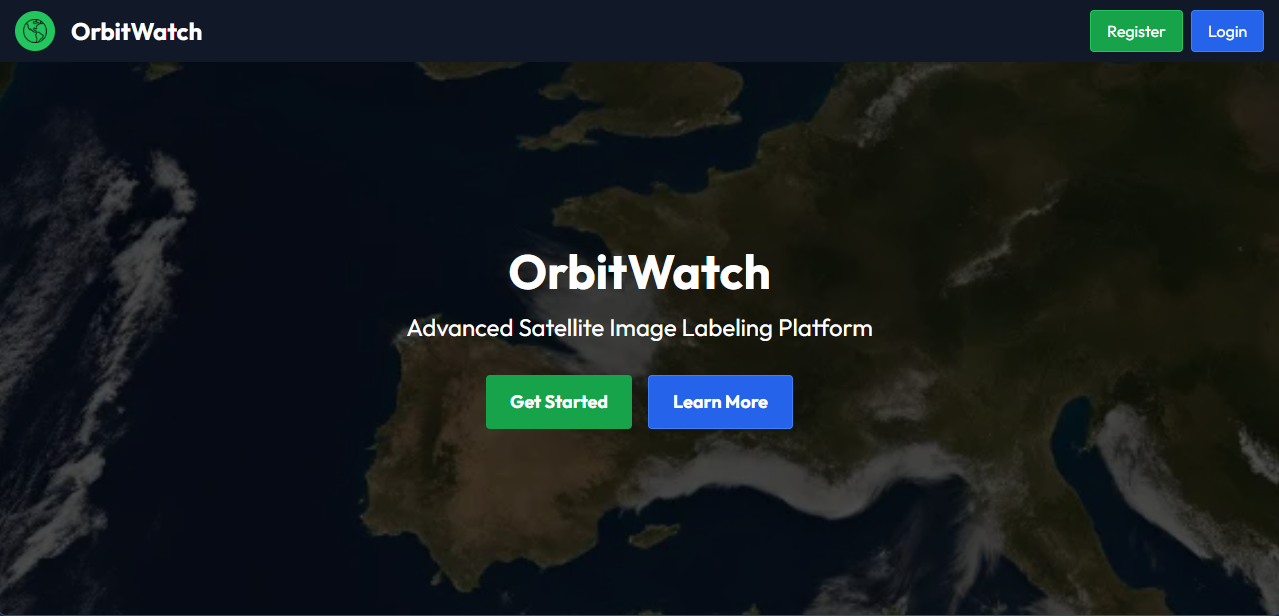
\includegraphics[width=\linewidth]{home.png}
    \caption{Home Page}
\end{figure}
\begin{figure}[H]
    \centering
    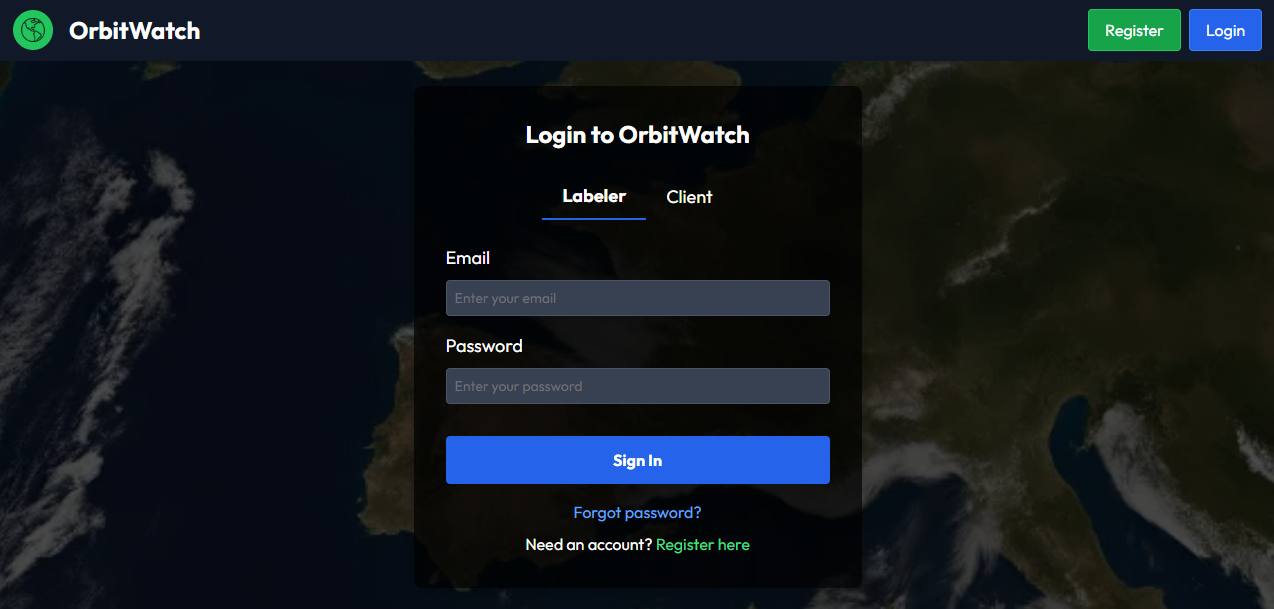
\includegraphics[width=\linewidth]{login.png}
    \caption{Login Page}
\end{figure}
\begin{figure}[H]
    \centering
    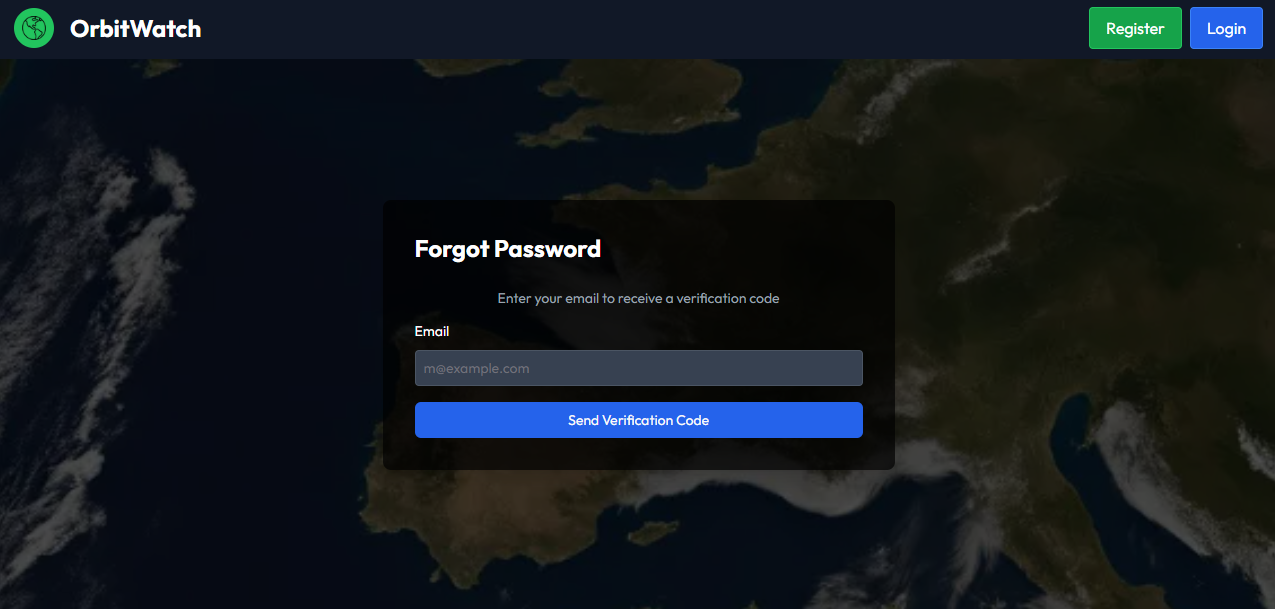
\includegraphics[width=\linewidth]{forgot_password.png}
    \caption{Forgot Password}
\end{figure}
\begin{figure}[H]
    \centering
    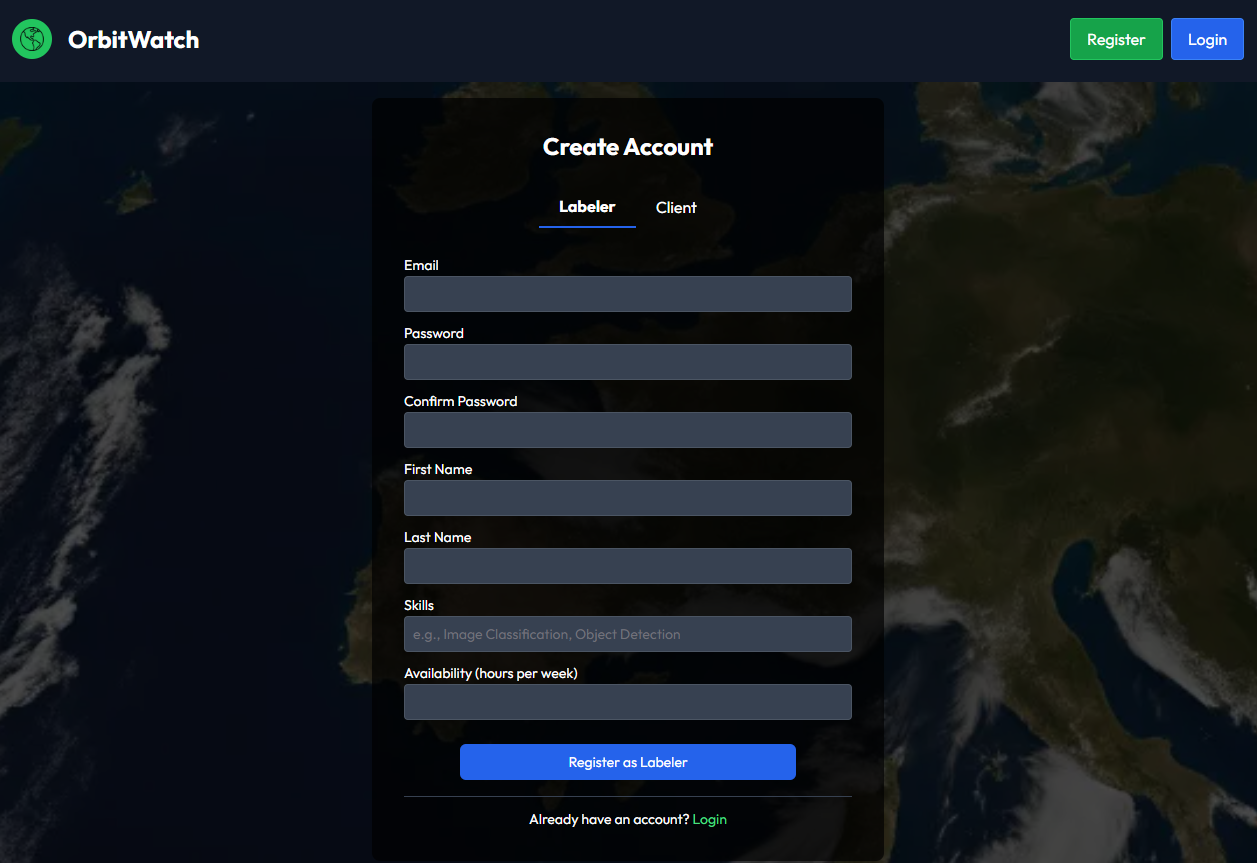
\includegraphics[width=\linewidth, height=10cm]{register.png}
    \caption{Register Page}
\end{figure}
\begin{figure}[H]
    \centering
    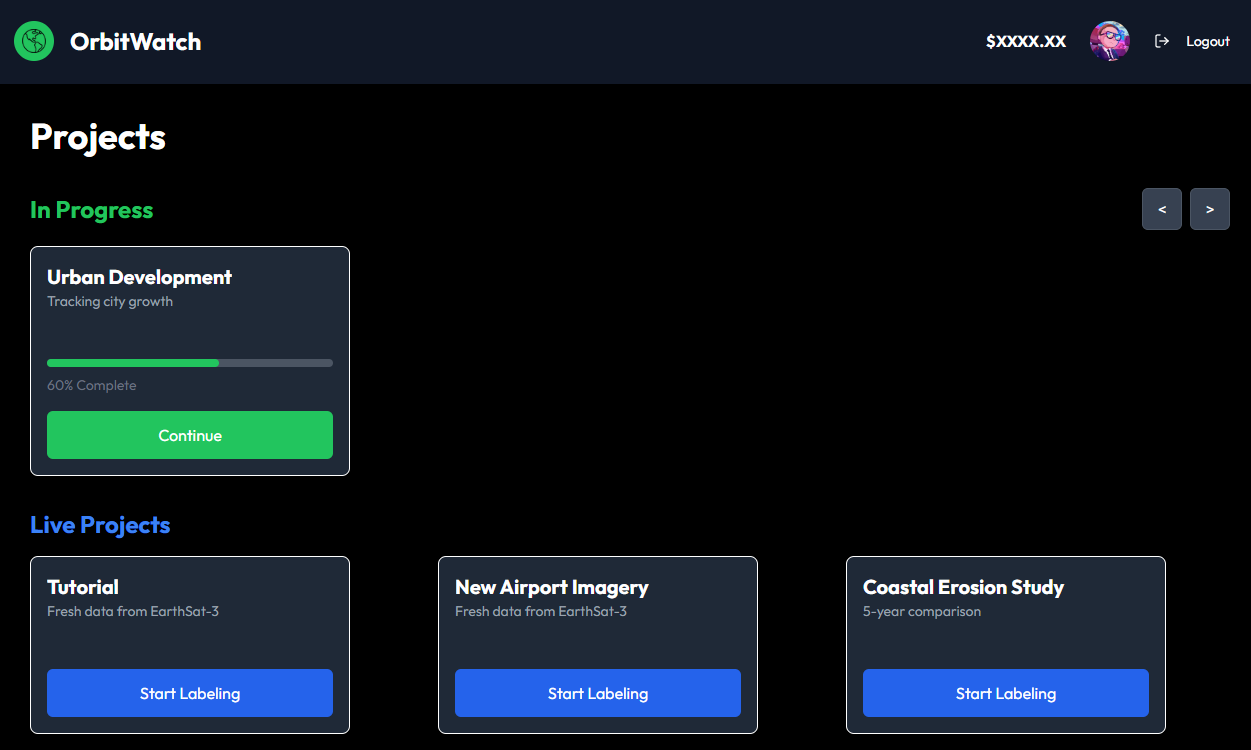
\includegraphics[width=\linewidth, height=8cm]{label_projects.png}
    \caption{Projects to Label Page}
\end{figure}
\begin{figure}[H]
    \centering
    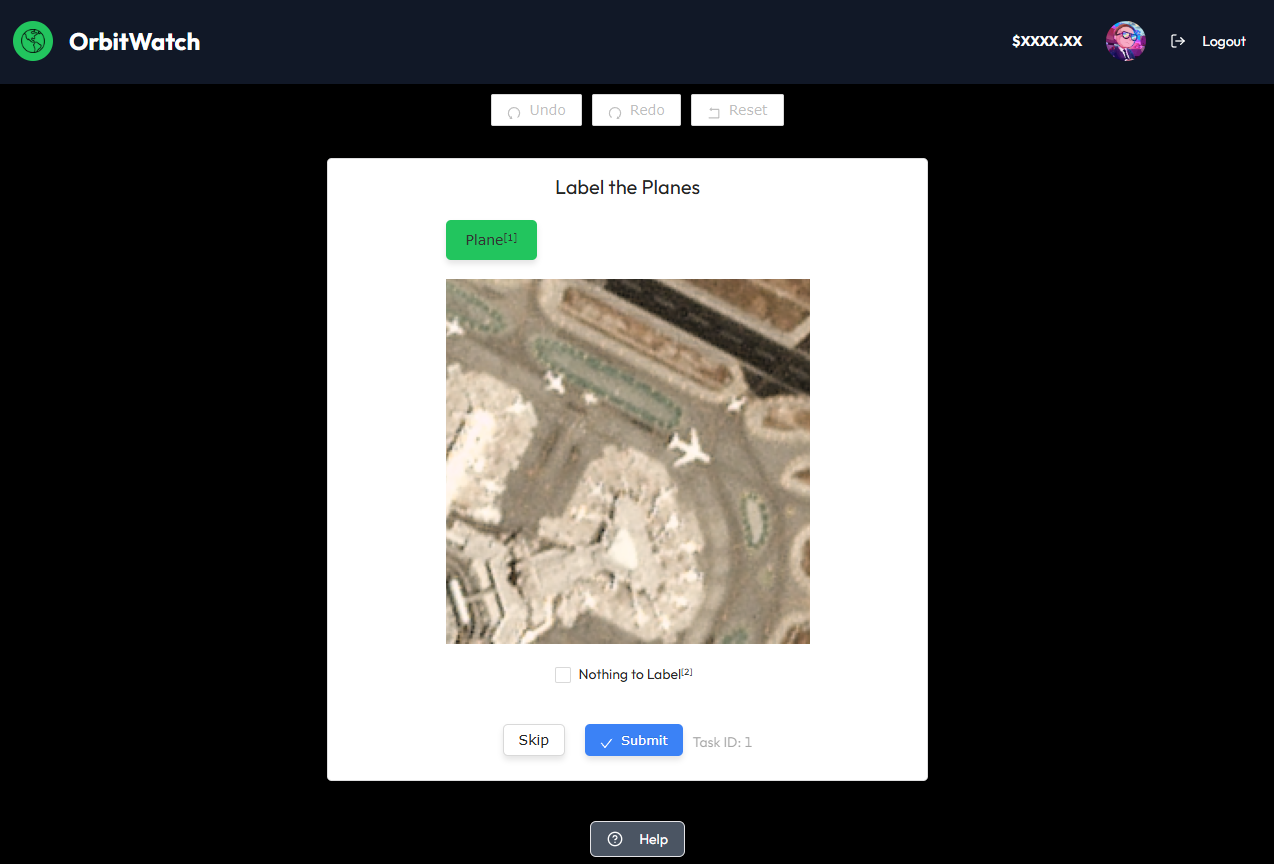
\includegraphics[scale=0.4]{label.png}
    \caption{Label Page}
\end{figure}
\begin{figure}[H]
    \centering
    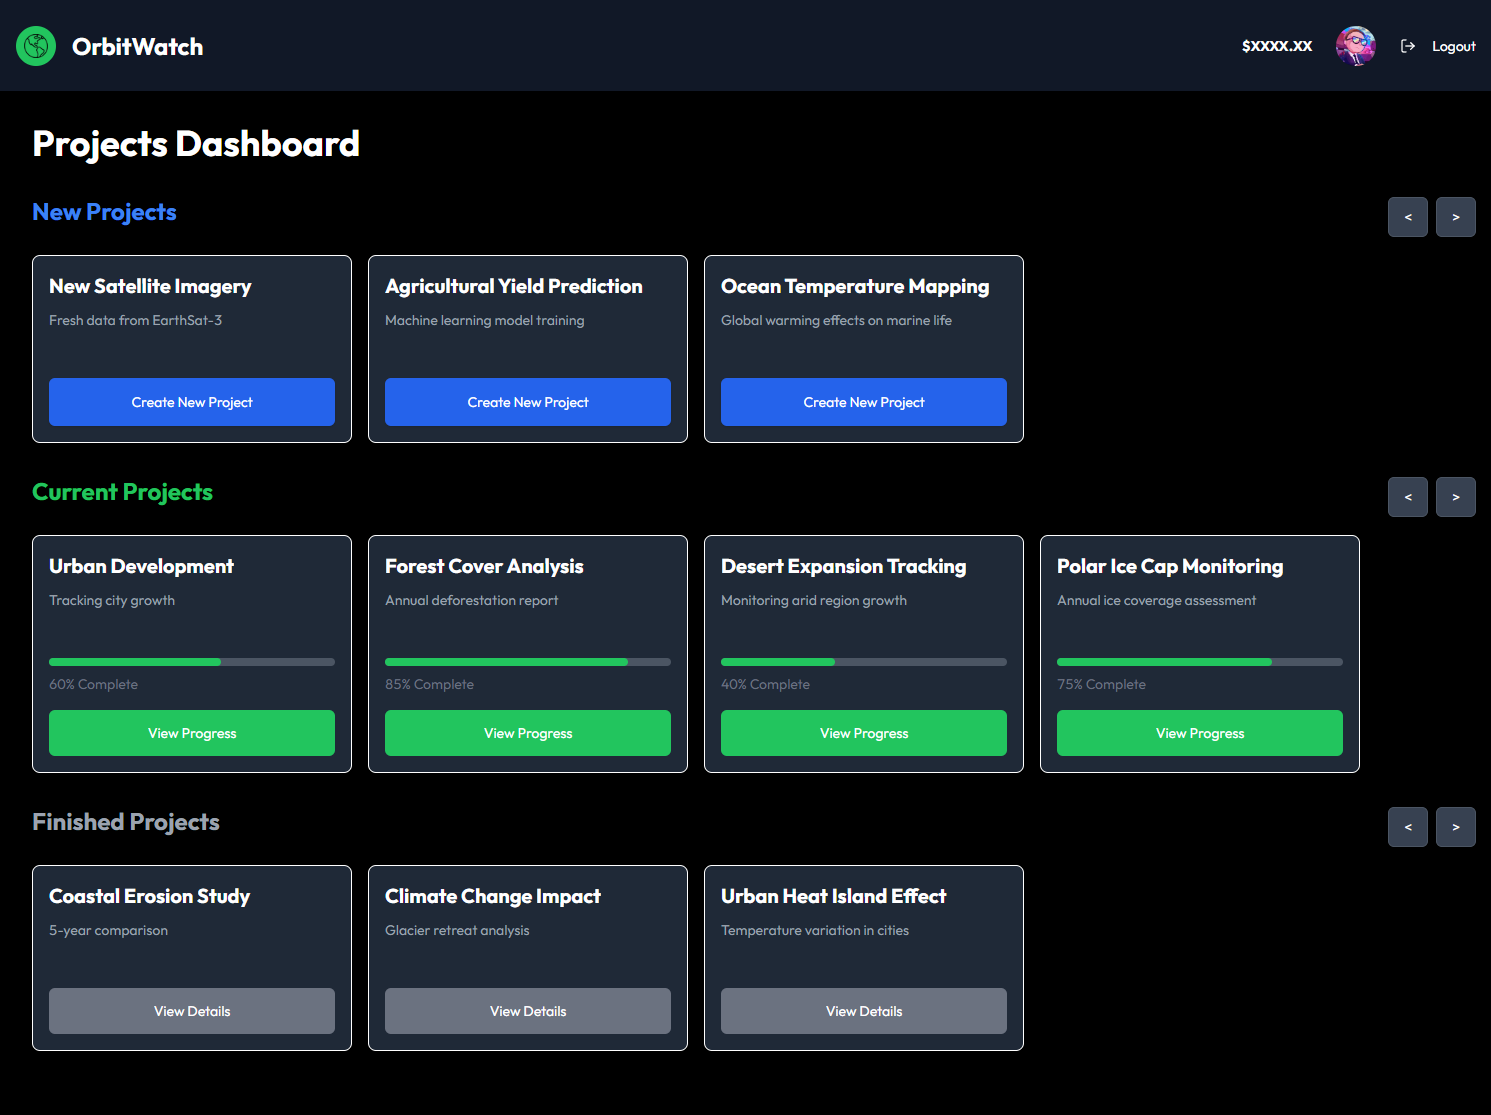
\includegraphics[scale=0.25]{client_projects.png}
    \caption{Client Projects Page}
\end{figure}
\begin{figure}[H]
    \centering
    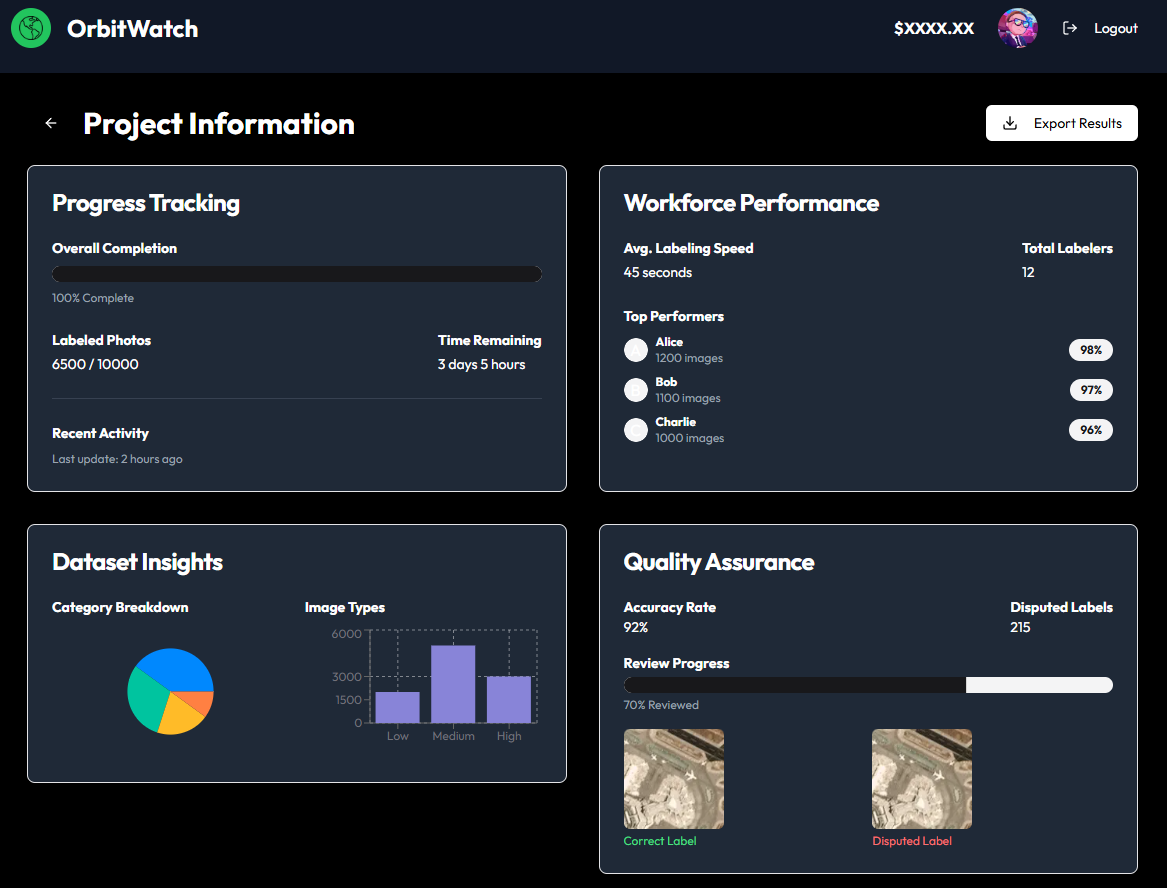
\includegraphics[scale=0.4]{project_stats.png}
    \caption{Project Status Page}
\end{figure}
\begin{figure}[H]
    \centering
    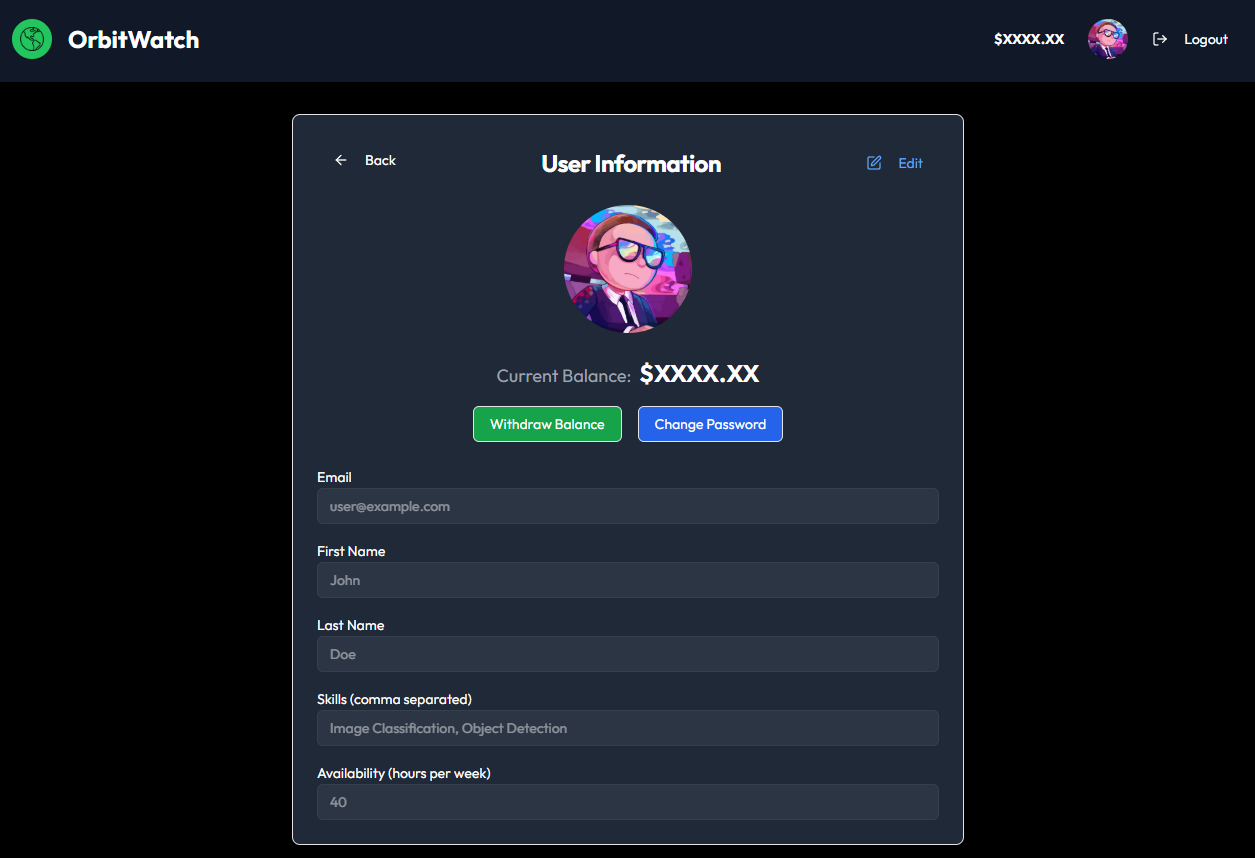
\includegraphics[scale=0.4]{user_info.png}
    \caption{User Information Page}
\end{figure}
\begin{figure}[H]
    \centering
    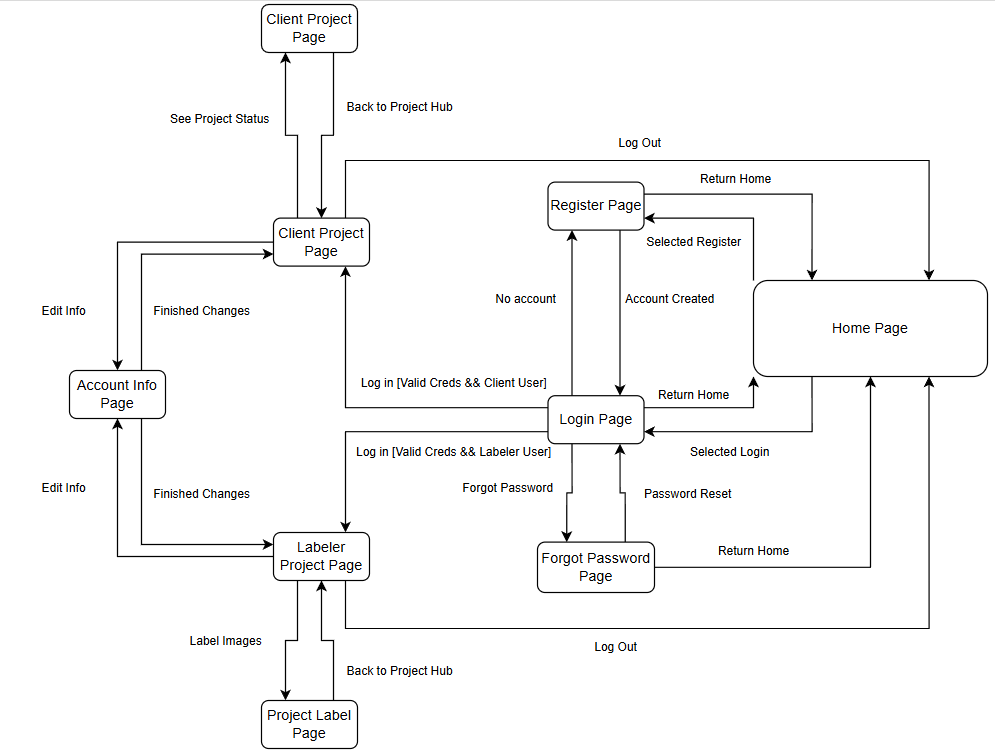
\includegraphics[width=\linewidth]{UI_flow.png}
    \caption{Page Flow Diagram}
\end{figure}

\section{Design of Communication Protocols}

\wss{If appropriate}

\section{Timeline}

\wss{Schedule of tasks and who is responsible}

\wss{You can point to GitHub if this information is included there}

\bibliographystyle {plainnat}
\bibliography{../../../refs/References}

\newpage{}

\end{document}